\documentclass[tikz,border=2pt]{standalone}
\usepackage{amsmath,amssymb}
\usepackage{pgfplots}
\pgfplotsset{compat=1.18}

\begin{document}
% Lognormal density (mu = 0, sigma = 0.5): X = e^Y with Y normal, so X > 0 and the density
% is right-skewed, with mode < median < mean.
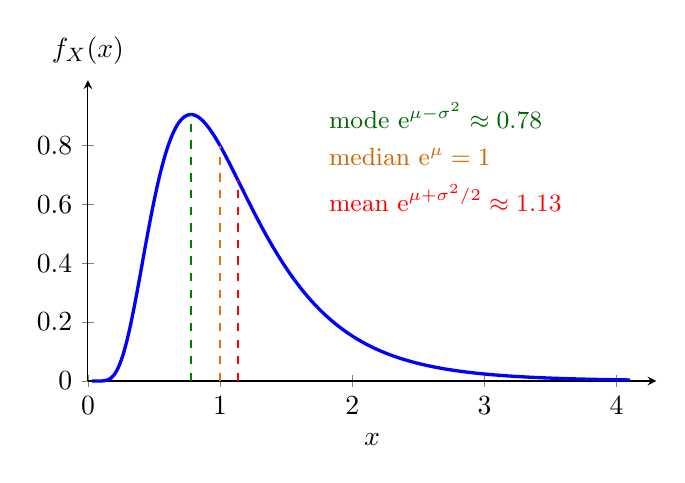
\begin{tikzpicture}
	\begin{axis}[
		axis lines=left, xmin=0, xmax=4.3, ymin=0, ymax=1.02,
		xtick={0,1,2,3,4}, ytick={0,0.2,0.4,0.6,0.8},
		xlabel={$x$}, ylabel={$f_X(x)$}, ylabel style={rotate=-90, anchor=south, at={(axis description cs:0,1.02)}},
		samples=200, smooth, width=8.8cm, height=5.4cm, clip=false
		]
		\addplot[blue, very thick, domain=0.03:4.1] {exp(-(ln(x))^2/(2*0.25))/(x*0.5*sqrt(2*pi))};
		\draw[green!50!black, dashed, thick] (axis cs:0.7788,0) -- (axis cs:0.7788,0.904);
		\draw[orange!90!black, dashed, thick] (axis cs:1,0) -- (axis cs:1,0.798);
		\draw[red, dashed, thick] (axis cs:1.1331,0) -- (axis cs:1.1331,0.683);
		\node[anchor=west, font=\small, green!40!black] at (axis cs:1.75,0.9) {mode $\mathrm{e}^{\mu-\sigma^2}\approx0.78$};
		\node[anchor=west, font=\small, orange!80!black] at (axis cs:1.75,0.76) {median $\mathrm{e}^{\mu}=1$};
		\node[anchor=west, font=\small, red] at (axis cs:1.75,0.62) {mean $\mathrm{e}^{\mu+\sigma^2/2}\approx1.13$};
	\end{axis}
	
\end{tikzpicture}
\end{document}
